% TrackPilot 补充材料中文对照译本（对应 supplement.tex）。仅供阅读和改写时对照，投稿以英文版为准。
% 表 S1--S14 来自 supp_tables_zh.tex，由 paper/make_supplement_zh.py 从 supp_tables.tex 生成（脚本核对数字不变）。
% 编译：cd paper && tectonic supplement_zh.tex（需要 XeTeX 和系统中文字体；Overleaf 上请选 XeLaTeX 并替换字体名）。
\documentclass[10pt]{article}
\usepackage[a4paper,margin=1.6cm,landscape]{geometry}
\usepackage{booktabs}
\usepackage{longtable}
\usepackage{float}
\usepackage{amsmath}
\usepackage{graphicx}
\usepackage{xeCJK}
\setCJKmainfont[AutoFakeBold=2.5,AutoFakeSlant=0.15]{STSong}
\setCJKsansfont[AutoFakeBold=2.5]{Hiragino Sans GB}
\setCJKmonofont{Hiragino Sans GB}
\xeCJKsetup{CJKspace=false}
\renewcommand{\figurename}{图}
\renewcommand{\tablename}{表}
\setlength{\LTcapwidth}{\textwidth}
\renewcommand{\thetable}{S\arabic{table}}
\title{补充材料\\[2pt]\large TrackPilot：用少量实测变异，为一种细胞类型选择可信的基因组基础模型轨道\\[2pt]
\normalsize（中文对照译本，仅供参考，以英文稿为准）}
\date{}
\begin{document}
\maketitle
\noindent 所有表格均由 \texttt{paper/make\_supplement.py} 从代码仓库 \texttt{results/a1} 下的结果表生成。Spearman 相关指留出变异的预测效应与实测效应之间的相关；差值在同一单位内配对（Kircher 为基因组区域；Siraj 为位点，两种细胞取平均）。场景：C1 已测绘（保留全部轨道），C2 仅有相近细胞（隐藏自身细胞系），C3 未测绘（隐藏自身及相近细胞类型）。v1 为预注册 Kircher 检验所用的早期版本（均匀先验），v2 为冻结的 \mbox{TrackPilot}。由 Siraj 数据派生的表格以 CC-BY-NC 4.0 许可发布。表~S6 分为两部分（S6a、S6b）。表~S15 的数字抄自其来源中注明的结果文件。表中的方法代号（如 disc、batch\_kb、matched\_cal）保留英文，含义见各表说明。

\begin{figure}[!ht]
\centering
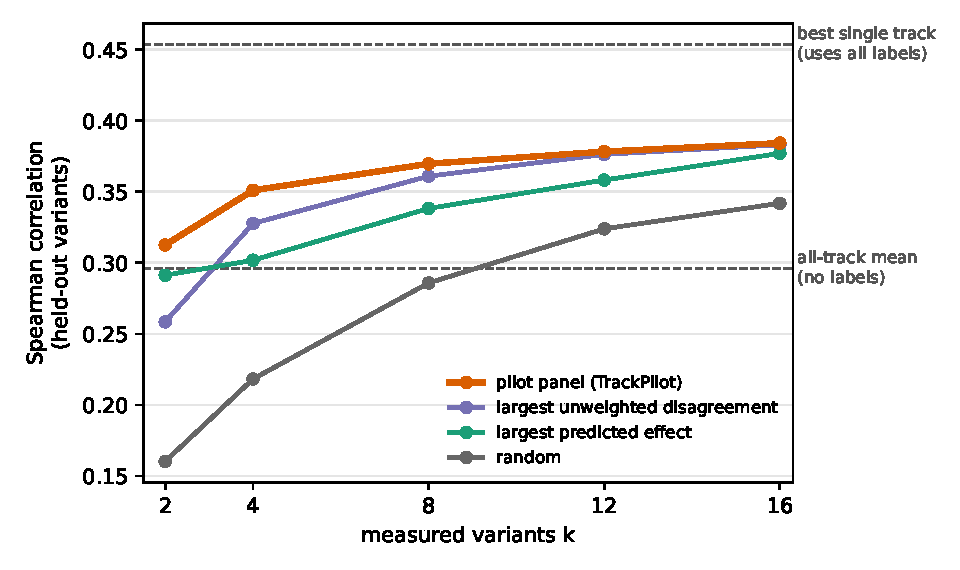
\includegraphics[width=0.55\textwidth]{figures/fig_s1_kircher_curve.pdf}
\renewcommand{\thefigure}{S1}
\caption{Kircher 检验集，隐藏自身及相近细胞类型：留出变异上的 Spearman 相关随实测变异数 $k$ 的变化，对 11 个检验区域取平均（同一区域的多个实验先取平均，与正文表~2 相同）。所有曲线使用同一轨道后验（预注册版本）。虚线：不用标签的全轨道平均，以及用全部标签选出的最佳单条轨道（作为参考）。来源：\texttt{paper/make\_fig\_s1.py}。}
\end{figure}

% Generated by paper/make_supplement_zh.py from supp_tables.tex; do not edit by hand.
\begin{table}[H]
\caption{Siraj 检验（125 个位点）：效应相对实测的参照寡核苷酸计算（主要分析），以及按原文发表的方式以元件全部寡核苷酸中心化（原始分析）。P1--P4 为预注册假设，在两种定义下全部成立。次要分析行给出位点平均差值及其 95\% bootstrap 区间。S3b 是改用相对参照的标签时新增的。}\label{tab:s1}
\centering\small
\begin{tabular}{llll}
\toprule
  & 统计量 & 相对参照 & 原文中心化 \\
\midrule
P1 $k=8$ & 平均 D（下界） & +0.010 (+0.005) & +0.010 (+0.005) \\
P2 $k=8$ & 受损位点（上界） & 3/125 (0.061) & 3/125 (0.061) \\
P1 $k=16$ & 平均 D（下界） & +0.019 (+0.013) & +0.020 (+0.013) \\
P2 $k=16$ & 受损位点（上界） & 1/125 (0.037) & 1/125 (0.037) \\
P3 $k=8$ & v2 $-$ 全轨道平均（$P$） & +0.047 ($P$=3e-12) & +0.048 ($P$=8e-13) \\
P4 $k=16$ & v2 $-$ 相近细胞平均（$P$） & +0.040 ($P$=3e-19) & +0.041 ($P$=1e-19) \\
S1 C1 k=8 & v2 试点组 $-$ v2 随机组 & +0.016 [+0.012 至 +0.021] & +0.018 [+0.013 至 +0.022] \\
S1 C3 k=8 & v2 试点组 $-$ v2 随机组 & +0.096 [+0.087 至 +0.104] & +0.093 [+0.085 至 +0.101] \\
S2 C1 k=8 & 同一试点组上 v2 $-$ meta\_ridge & +0.007 [+0.003 至 +0.011] & +0.008 [+0.004 至 +0.012] \\
S3 C1 k=8 & matched\_cal（随机组）$-$ 匹配轨道 & $-$0.082 [$-$0.090 至 $-$0.075] & $-$0.079 [$-$0.086 至 $-$0.072] \\
S3b C1 k=8 & matched\_cal（试点组）$-$ 匹配轨道 & $-$0.010 [$-$0.015 至 $-$0.006] & -- \\
S5 C1 k=8 & 族先验 $-$ 均匀先验 & $-$0.002 [$-$0.004 至 $-$0.000] & $-$0.002 [$-$0.003 至 +0.000] \\
S7 HEPG2 C1 k=8 & v2 $-$ 匹配轨道 & +0.016 [+0.007 至 +0.026] & +0.017 [+0.007 至 +0.026] \\
S7 HEPG2 C3 k=8 & v2 $-$ 全轨道平均 & +0.050 [+0.029 至 +0.074] & +0.052 [+0.031 至 +0.076] \\
S7 K562 C1 k=8 & v2 $-$ 匹配轨道 & +0.003 [$-$0.001 至 +0.007] & +0.003 [$-$0.002 至 +0.007] \\
S7 K562 C3 k=8 & v2 $-$ 全轨道平均 & +0.043 [+0.029 至 +0.058] & +0.044 [+0.031 至 +0.059] \\
\bottomrule
\end{tabular}
\end{table}

\begin{table}[H]
\caption{方向准确率（事后分析）：留出的显著变异（$P<10^{-5}$，$|\text{效应}|\ge0.1$）中预测方向正确的比例。带标签的方法使用后验平均预测；“去偏移”表示去掉拟合的偏移（诊断用）。区间：按单位做 95\% bootstrap；最后一列为前者更好/更差的单位数。disc：试点变异组；random：随机组；matched：匹配轨道平均；all\_mean：全轨道平均；related：相近细胞平均；matched\_cal：对匹配轨道平均做仿射重拟合；@ 后为标签数。}\label{tab:s2}
\centering\small
\begin{tabular}{llllrrrrll}
\toprule
数据集 & 对比 & 前者 & 后者 & $n$ & 准确率 1 & 准确率 2 & 差值 & 95\% CI & +/$-$ \\
\midrule
Siraj & P1 & disc@8 & matched@0 & 125 & 0.874 & 0.867 & +0.007 & $-$0.010 至 +0.024 & 63/60 \\
Siraj & P1 (S4) & disc@16 & matched@0 & 125 & 0.886 & 0.867 & +0.019 & +0.001 至 +0.037 & 66/57 \\
Siraj & P3 & disc@8 & all\_mean@0 & 125 & 0.864 & 0.809 & +0.055 & +0.032 至 +0.078 & 76/48 \\
Siraj & P4 & disc@16 & related@0 & 125 & 0.873 & 0.834 & +0.039 & +0.020 至 +0.057 & 80/45 \\
Siraj & S1 & disc@8 & random@8 & 125 & 0.864 & 0.789 & +0.074 & +0.061 至 +0.089 & 107/18 \\
Siraj & S3 & random+matched\_cal@8 & matched@0 & 125 & 0.817 & 0.867 & $-$0.050 & $-$0.068 至 $-$0.032 & 30/95 \\
Siraj & S3b & disc+matched\_cal@8 & matched@0 & 125 & 0.865 & 0.867 & $-$0.002 & $-$0.021 至 +0.017 & 57/66 \\
Kircher（v1） & H1 & disc@8 & random@8 & 11 & 0.675 & 0.694 & $-$0.018 & $-$0.105 至 +0.042 & 7/4 \\
Kircher（v1） & H2 & disc@8 & all\_mean@0 & 11 & 0.675 & 0.774 & $-$0.099 & $-$0.267 至 +0.046 & 4/7 \\
Kircher（v2） & v2 C1 k=8 & disc@8 & matched@0 & 11 & 0.706 & 0.839 & $-$0.133 & $-$0.264 至 $-$0.026 & 2/9 \\
Kircher（v2） & v2 C1 k=16 & disc@16 & matched@0 & 11 & 0.730 & 0.839 & $-$0.108 & $-$0.230 至 $-$0.010 & 3/8 \\
Kircher（v2，去偏移） & v2 C1 k=8 & disc@8 & matched@0 & 11 & 0.768 & 0.839 & $-$0.071 & $-$0.207 至 +0.011 & 5/4 \\
Kircher（v2，去偏移） & v2 C1 k=16 & disc@16 & matched@0 & 11 & 0.790 & 0.839 & $-$0.048 & $-$0.158 至 +0.027 & 6/3 \\
Kircher（v2，去偏移） & v2 C3 k=8 & disc@8 & all\_mean@0 & 11 & 0.743 & 0.774 & $-$0.031 & $-$0.188 至 +0.107 & 8/3 \\
Kircher（v2，去偏移） & v2 C3 k=8 对随机 & disc@8 & random@8 & 11 & 0.743 & 0.700 & +0.042 & $-$0.029 至 +0.101 & 9/2 \\
Kircher（v2） & v2 C3 k=8 & disc@8 & all\_mean@0 & 11 & 0.694 & 0.774 & $-$0.079 & $-$0.232 至 +0.055 & 4/7 \\
Kircher（v2） & v2 C3 k=8 对随机 & disc@8 & random@8 & 11 & 0.694 & 0.693 & +0.002 & $-$0.066 至 +0.052 & 8/3 \\
\bottomrule
\end{tabular}
\end{table}

\begin{table}[H]
\caption{为每个位点换用留出其基因组折的 AlphaGenome 检查点后，重做 Siraj 检验（标签相对参照寡核苷酸）。各列为蒸馏检查点（ALL\_FOLDS）和留出检查点下的预注册对比，以及配对变化量及其按位点的 95\% bootstrap 区间。}\label{tab:s3}
\centering\small
\begin{tabular}{lrrll}
\toprule
假设 & ALL\_FOLDS & 留出折 & 变化 [95\% CI] & 判定 \\
\midrule
P1 $k=8$ & +0.010 & +0.024 & +0.014 [+0.008 至 +0.022] & 成立 \\
P1 $k=16$ & +0.019 & +0.037 & +0.018 [+0.009 至 +0.027] & 成立 \\
P3 $k=8$ & +0.047 & +0.050 & +0.003 [$-$0.006 至 +0.013] & 成立 \\
P4 $k=16$ & +0.040 & +0.053 & +0.013 [+0.006 至 +0.021] & 成立 \\
P2 $k=8$ & 3/125 受损 & 1/125 受损 & -- & 成立 \\
P2 $k=16$ & 1/125 受损 & 1/125 受损 & -- & 成立 \\
\bottomrule
\end{tabular}
\end{table}

{\small\begin{longtable}{llrlrrll}
\caption{选点方式比较（事后分析；推断使用冻结的 v2，50 次重复）。Siraj 为场景 C1--C3；Kircher 为检验区域，分为保留匹配轨道（deploy）和没有锚点（no\_anchor）。disc：逐个选择的试点变异组；batch\_kb：测量前一轮选完；disc\_static：不随标签更新的先验分歧；eig：期望信息增益；high\_effect：预测效应最大；disagree：未加权分歧最大。判读：95\% 区间落在 $\pm0.02$ 以内为等价；整体高于或低于 0 为前者或后者更好。}\label{tab:s4}\\
\toprule
数据 & 场景 & $k$ & 对比 & $n$ & 均值 & 95\% CI & 判读 \\
\midrule
\endfirsthead
\toprule
数据 & 场景 & $k$ & 对比 & $n$ & 均值 & 95\% CI & 判读 \\
\midrule
\endhead
Siraj & C1 & 8 & disc $-$ batch\_kb & 125 & +0.002 & $-$0.000 至 +0.004 & 等价 \\
Siraj & C2 & 8 & disc $-$ batch\_kb & 125 & +0.005 & +0.003 至 +0.007 & 等价 \\
Siraj & C3 & 8 & disc $-$ batch\_kb & 125 & +0.004 & +0.002 至 +0.006 & 等价 \\
Siraj & C1 & 8 & disc $-$ disc\_static & 125 & +0.007 & +0.004 至 +0.012 & 等价 \\
Siraj & C2 & 8 & disc $-$ disc\_static & 125 & +0.014 & +0.008 至 +0.020 & 前者更好 \\
Siraj & C3 & 8 & disc $-$ disc\_static & 125 & +0.023 & +0.017 至 +0.029 & 前者更好 \\
Siraj & C1 & 8 & eig $-$ disc & 125 & +0.000 & $-$0.001 至 +0.002 & 等价 \\
Siraj & C2 & 8 & eig $-$ disc & 125 & +0.001 & $-$0.000 至 +0.002 & 等价 \\
Siraj & C3 & 8 & eig $-$ disc & 125 & +0.000 & $-$0.001 至 +0.002 & 等价 \\
Siraj & C1 & 8 & batch\_kb $-$ disc\_static & 125 & +0.005 & +0.002 至 +0.010 & 等价 \\
Siraj & C2 & 8 & batch\_kb $-$ disc\_static & 125 & +0.009 & +0.004 至 +0.014 & 等价 \\
Siraj & C3 & 8 & batch\_kb $-$ disc\_static & 125 & +0.019 & +0.014 至 +0.025 & 前者更好 \\
Siraj & C1 & 8 & disc $-$ high\_effect & 125 & +0.010 & +0.005 至 +0.016 & 等价 \\
Siraj & C2 & 8 & disc $-$ high\_effect & 125 & +0.017 & +0.011 至 +0.024 & 前者更好 \\
Siraj & C3 & 8 & disc $-$ high\_effect & 125 & +0.028 & +0.020 至 +0.035 & 前者更好 \\
Siraj & C1 & 8 & disc $-$ disagree & 125 & +0.013 & +0.008 至 +0.018 & 等价 \\
Siraj & C2 & 8 & disc $-$ disagree & 125 & +0.017 & +0.011 至 +0.023 & 前者更好 \\
Siraj & C3 & 8 & disc $-$ disagree & 125 & +0.032 & +0.024 至 +0.041 & 前者更好 \\
Siraj & C1 & 16 & disc $-$ batch\_kb & 125 & +0.004 & +0.002 至 +0.007 & 等价 \\
Siraj & C2 & 16 & disc $-$ batch\_kb & 125 & +0.008 & +0.006 至 +0.010 & 等价 \\
Siraj & C3 & 16 & disc $-$ batch\_kb & 125 & +0.006 & +0.004 至 +0.009 & 等价 \\
Siraj & C1 & 16 & disc $-$ disc\_static & 125 & +0.009 & +0.005 至 +0.013 & 等价 \\
Siraj & C2 & 16 & disc $-$ disc\_static & 125 & +0.016 & +0.013 至 +0.021 & 前者更好 \\
Siraj & C3 & 16 & disc $-$ disc\_static & 125 & +0.016 & +0.012 至 +0.021 & 前者更好 \\
Siraj & C1 & 16 & eig $-$ disc & 125 & +0.001 & +0.000 至 +0.002 & 等价 \\
Siraj & C2 & 16 & eig $-$ disc & 125 & +0.001 & +0.000 至 +0.002 & 等价 \\
Siraj & C3 & 16 & eig $-$ disc & 125 & +0.000 & $-$0.001 至 +0.001 & 等价 \\
Siraj & C1 & 16 & batch\_kb $-$ disc\_static & 125 & +0.005 & +0.002 至 +0.009 & 等价 \\
Siraj & C2 & 16 & batch\_kb $-$ disc\_static & 125 & +0.008 & +0.005 至 +0.012 & 等价 \\
Siraj & C3 & 16 & batch\_kb $-$ disc\_static & 125 & +0.010 & +0.006 至 +0.014 & 等价 \\
Siraj & C1 & 16 & disc $-$ high\_effect & 125 & +0.012 & +0.007 至 +0.018 & 等价 \\
Siraj & C2 & 16 & disc $-$ high\_effect & 125 & +0.023 & +0.018 至 +0.029 & 前者更好 \\
Siraj & C3 & 16 & disc $-$ high\_effect & 125 & +0.027 & +0.021 至 +0.033 & 前者更好 \\
Siraj & C1 & 16 & disc $-$ disagree & 125 & +0.011 & +0.006 至 +0.016 & 等价 \\
Siraj & C2 & 16 & disc $-$ disagree & 125 & +0.015 & +0.011 至 +0.020 & 前者更好 \\
Siraj & C3 & 16 & disc $-$ disagree & 125 & +0.020 & +0.016 至 +0.025 & 前者更好 \\
Kircher & deploy & 8 & disc $-$ batch\_kb & 11 & +0.004 & $-$0.001 至 +0.009 & 等价 \\
Kircher & no\_anchor & 8 & disc $-$ batch\_kb & 11 & +0.003 & $-$0.004 至 +0.010 & 等价 \\
Kircher & deploy & 8 & disc $-$ disc\_static & 11 & +0.006 & +0.000 至 +0.011 & 等价 \\
Kircher & no\_anchor & 8 & disc $-$ disc\_static & 11 & +0.015 & $-$0.001 至 +0.035 & 未定 \\
Kircher & deploy & 8 & eig $-$ disc & 11 & +0.003 & +0.001 至 +0.005 & 等价 \\
Kircher & no\_anchor & 8 & eig $-$ disc & 11 & +0.002 & $-$0.001 至 +0.005 & 等价 \\
Kircher & deploy & 8 & batch\_kb $-$ disc\_static & 11 & +0.002 & $-$0.003 至 +0.006 & 等价 \\
Kircher & no\_anchor & 8 & batch\_kb $-$ disc\_static & 11 & +0.012 & +0.001 至 +0.029 & 前者更好 \\
Kircher & deploy & 8 & disc $-$ high\_effect & 11 & +0.004 & $-$0.007 至 +0.017 & 等价 \\
Kircher & no\_anchor & 8 & disc $-$ high\_effect & 11 & +0.029 & +0.001 至 +0.059 & 前者更好 \\
Kircher & deploy & 8 & disc $-$ disagree & 11 & +0.005 & $-$0.009 至 +0.023 & 未定 \\
Kircher & no\_anchor & 8 & disc $-$ disagree & 11 & +0.019 & $-$0.003 至 +0.041 & 未定 \\
Kircher & deploy & 16 & disc $-$ batch\_kb & 11 & +0.005 & +0.000 至 +0.012 & 等价 \\
Kircher & no\_anchor & 16 & disc $-$ batch\_kb & 11 & +0.008 & +0.002 至 +0.013 & 等价 \\
Kircher & deploy & 16 & disc $-$ disc\_static & 11 & +0.020 & +0.000 至 +0.048 & 前者更好 \\
Kircher & no\_anchor & 16 & disc $-$ disc\_static & 11 & +0.013 & $-$0.002 至 +0.028 & 未定 \\
Kircher & deploy & 16 & eig $-$ disc & 11 & +0.004 & +0.001 至 +0.007 & 等价 \\
Kircher & no\_anchor & 16 & eig $-$ disc & 11 & +0.002 & $-$0.001 至 +0.006 & 等价 \\
Kircher & deploy & 16 & batch\_kb $-$ disc\_static & 11 & +0.015 & $-$0.003 至 +0.043 & 未定 \\
Kircher & no\_anchor & 16 & batch\_kb $-$ disc\_static & 11 & +0.005 & $-$0.011 至 +0.018 & 等价 \\
Kircher & deploy & 16 & disc $-$ high\_effect & 11 & +0.022 & $-$0.004 至 +0.055 & 未定 \\
Kircher & no\_anchor & 16 & disc $-$ high\_effect & 11 & +0.001 & $-$0.021 至 +0.023 & 未定 \\
Kircher & deploy & 16 & disc $-$ disagree & 11 & +0.020 & +0.002 至 +0.041 & 前者更好 \\
Kircher & no\_anchor & 16 & disc $-$ disagree & 11 & +0.008 & $-$0.004 至 +0.019 & 等价 \\
\bottomrule
\end{longtable}}

{\small\begin{longtable}{llrlrrlrl}
\caption{CODA 式与 MODEL SELECTOR 式基线（事后分析；50 次重复）。两者都使用校准似然、不使用元数据、按信息增益选点；CODA 使用共识先验（$\kappa=10$，在开发元件上固定），MODEL SELECTOR 使用均匀先验（$\kappa=0$）。“单条轨道”：最可能的轨道，即这些方法本身的输出；“平均”：它们的后验平均。“+”：前者更好的单位数。}\label{tab:s5}\\
\toprule
数据 & 场景 & $k$ & 对比 & $n$ & 均值 & 95\% CI & + & 判读 \\
\midrule
\endfirsthead
\toprule
数据 & 场景 & $k$ & 对比 & $n$ & 均值 & 95\% CI & + & 判读 \\
\midrule
\endhead
Siraj & C1 & 8 & v2 $-$ coda （单条轨道） & 125 & +0.075 & +0.062 至 +0.089 & 111 & 前者更好 \\
Siraj & C1 & 8 & v2 $-$ model\_selector （单条轨道） & 125 & +0.074 & +0.064 至 +0.084 & 118 & 前者更好 \\
Siraj & C1 & 8 & coda：平均 $-$ 单条轨道 & 125 & +0.016 & +0.012 至 +0.021 & 99 & 前者更好 \\
Siraj & C1 & 8 & v2 $-$ coda （平均） & 125 & +0.059 & +0.045 至 +0.072 & 105 & 前者更好 \\
Siraj & C1 & 16 & v2 $-$ coda （单条轨道） & 125 & +0.045 & +0.038 至 +0.054 & 111 & 前者更好 \\
Siraj & C1 & 16 & v2 $-$ model\_selector （单条轨道） & 125 & +0.042 & +0.035 至 +0.049 & 112 & 前者更好 \\
Siraj & C1 & 16 & coda：平均 $-$ 单条轨道 & 125 & +0.009 & +0.005 至 +0.012 & 92 & 等价 \\
Siraj & C1 & 16 & v2 $-$ coda （平均） & 125 & +0.037 & +0.028 至 +0.045 & 107 & 前者更好 \\
Siraj & C2 & 8 & v2 $-$ coda （单条轨道） & 125 & +0.029 & +0.019 至 +0.039 & 88 & 前者更好 \\
Siraj & C2 & 8 & v2 $-$ model\_selector （单条轨道） & 125 & +0.036 & +0.029 至 +0.045 & 99 & 前者更好 \\
Siraj & C2 & 8 & coda：平均 $-$ 单条轨道 & 125 & +0.018 & +0.014 至 +0.022 & 103 & 前者更好 \\
Siraj & C2 & 8 & v2 $-$ coda （平均） & 125 & +0.011 & +0.002 至 +0.021 & 70 & 前者更好 \\
Siraj & C2 & 16 & v2 $-$ coda （单条轨道） & 125 & +0.017 & +0.010 至 +0.023 & 88 & 前者更好 \\
Siraj & C2 & 16 & v2 $-$ model\_selector （单条轨道） & 125 & +0.018 & +0.013 至 +0.023 & 90 & 前者更好 \\
Siraj & C2 & 16 & coda：平均 $-$ 单条轨道 & 125 & +0.012 & +0.009 至 +0.015 & 98 & 等价 \\
Siraj & C2 & 16 & v2 $-$ coda （平均） & 125 & +0.005 & $-$0.001 至 +0.011 & 70 & 等价 \\
Siraj & C3 & 8 & v2 $-$ coda （单条轨道） & 125 & +0.034 & +0.027 至 +0.042 & 106 & 前者更好 \\
Siraj & C3 & 8 & v2 $-$ model\_selector （单条轨道） & 125 & +0.044 & +0.039 至 +0.049 & 121 & 前者更好 \\
Siraj & C3 & 8 & coda：平均 $-$ 单条轨道 & 125 & +0.017 & +0.013 至 +0.021 & 105 & 前者更好 \\
Siraj & C3 & 8 & v2 $-$ coda （平均） & 125 & +0.018 & +0.011 至 +0.024 & 83 & 前者更好 \\
Siraj & C3 & 16 & v2 $-$ coda （单条轨道） & 125 & +0.028 & +0.023 至 +0.034 & 114 & 前者更好 \\
Siraj & C3 & 16 & v2 $-$ model\_selector （单条轨道） & 125 & +0.030 & +0.026 至 +0.034 & 115 & 前者更好 \\
Siraj & C3 & 16 & coda：平均 $-$ 单条轨道 & 125 & +0.012 & +0.009 至 +0.015 & 98 & 等价 \\
Siraj & C3 & 16 & v2 $-$ coda （平均） & 125 & +0.016 & +0.012 至 +0.021 & 93 & 前者更好 \\
Kircher & C1 & 8 & v2 $-$ coda （单条轨道） & 11 & +0.082 & +0.006 至 +0.149 & 8 & 前者更好 \\
Kircher & C1 & 8 & v2 $-$ model\_selector （单条轨道） & 11 & +0.070 & $-$0.003 至 +0.138 & 8 & 未定 \\
Kircher & C1 & 8 & coda：平均 $-$ 单条轨道 & 11 & +0.026 & +0.015 至 +0.037 & 9 & 前者更好 \\
Kircher & C1 & 8 & v2 $-$ coda （平均） & 11 & +0.056 & $-$0.019 至 +0.120 & 8 & 未定 \\
Kircher & C1 & 16 & v2 $-$ coda （单条轨道） & 11 & +0.056 & +0.013 至 +0.099 & 9 & 前者更好 \\
Kircher & C1 & 16 & v2 $-$ model\_selector （单条轨道） & 11 & +0.061 & +0.013 至 +0.108 & 7 & 前者更好 \\
Kircher & C1 & 16 & coda：平均 $-$ 单条轨道 & 11 & +0.017 & +0.005 至 +0.029 & 7 & 前者更好 \\
Kircher & C1 & 16 & v2 $-$ coda （平均） & 11 & +0.039 & $-$0.007 至 +0.081 & 8 & 未定 \\
Kircher & C3 & 8 & v2 $-$ coda （单条轨道） & 11 & +0.051 & +0.018 至 +0.087 & 8 & 前者更好 \\
Kircher & C3 & 8 & v2 $-$ model\_selector （单条轨道） & 11 & +0.042 & +0.005 至 +0.075 & 8 & 前者更好 \\
Kircher & C3 & 8 & coda：平均 $-$ 单条轨道 & 11 & +0.025 & +0.015 至 +0.034 & 9 & 前者更好 \\
Kircher & C3 & 8 & v2 $-$ coda （平均） & 11 & +0.026 & $-$0.005 至 +0.059 & 7 & 未定 \\
Kircher & C3 & 16 & v2 $-$ coda （单条轨道） & 11 & +0.030 & +0.015 至 +0.045 & 9 & 前者更好 \\
Kircher & C3 & 16 & v2 $-$ model\_selector （单条轨道） & 11 & +0.028 & +0.002 至 +0.051 & 8 & 前者更好 \\
Kircher & C3 & 16 & coda：平均 $-$ 单条轨道 & 11 & +0.019 & +0.007 至 +0.032 & 8 & 前者更好 \\
Kircher & C3 & 16 & v2 $-$ coda （平均） & 11 & +0.011 & $-$0.008 至 +0.028 & 6 & 未定 \\
\bottomrule
\end{longtable}}

\renewcommand{\thetable}{S6a}

\begin{table}[H]
\caption{信息增益（EIG）收敛检查（事后分析）之覆盖率：保留的假设所占的后验概率，按单位取中位数（括号内为最小值），分别给出第一步和 $k=8$ 变异组八步中的最低值。E0：最可能的 100 个假设，96 个积分点（表 S4 使用的设置）；E1：300 个假设；E2（未列出）每一步都保留 $\ge$99\% 的概率，使用 192 个积分点。}\label{tab:s6a}
\centering\small
\begin{tabular}{llrrrr}
\toprule
数据 & 场景 & E0 第一步 & E0 最低 & E1 第一步 & E1 最低 \\
\midrule
Siraj & C1 & 0.98 (0.96) & 0.93 (0.79) & 0.99 (0.98) & 0.98 (0.91) \\
Siraj & C2 & 0.98 (0.96) & 0.94 (0.76) & 0.99 (0.98) & 0.98 (0.91) \\
Siraj & C3 & 0.61 (0.23) & 0.60 (0.23) & 0.87 (0.66) & 0.86 (0.66) \\
Kircher & deploy & 0.97 (0.97) & 0.95 (0.79) & 0.99 (0.99) & 0.98 (0.92) \\
Kircher & no\_anchor & 0.49 (0.32) & 0.49 (0.32) & 0.84 (0.76) & 0.84 (0.76) \\
\bottomrule
\end{tabular}
\end{table}

\addtocounter{table}{-1}\renewcommand{\thetable}{S6b}

{\small\begin{longtable}{llrlrrll}
\caption{信息增益收敛检查之准确度：后验平均预测的 Spearman 相关差值（相同的变异池和 50 次重复；按单位做 95\% bootstrap 区间）。}\label{tab:s6b}\\
\toprule
数据 & 场景 & $k$ & 对比 & $n$ & 均值 & 95\% CI & 判读 \\
\midrule
\endfirsthead
\toprule
数据 & 场景 & $k$ & 对比 & $n$ & 均值 & 95\% CI & 判读 \\
\midrule
\endhead
Siraj & C1 & 8 & E2 $-$ E0 & 125 & $-$0.0002 & $-$0.001 至 +0.001 & 等价 \\
Siraj & C2 & 8 & E2 $-$ E0 & 125 & $-$0.0002 & $-$0.001 至 +0.001 & 等价 \\
Siraj & C3 & 8 & E2 $-$ E0 & 125 & +0.0004 & $-$0.001 至 +0.001 & 等价 \\
Siraj & C1 & 8 & E2 $-$ disc & 125 & $-$0.0000 & $-$0.001 至 +0.001 & 等价 \\
Siraj & C2 & 8 & E2 $-$ disc & 125 & +0.0006 & $-$0.001 至 +0.002 & 等价 \\
Siraj & C3 & 8 & E2 $-$ disc & 125 & +0.0007 & $-$0.001 至 +0.002 & 等价 \\
Siraj & C1 & 8 & E0 $-$ disc & 125 & +0.0002 & $-$0.001 至 +0.002 & 等价 \\
Siraj & C2 & 8 & E0 $-$ disc & 125 & +0.0008 & $-$0.000 至 +0.002 & 等价 \\
Siraj & C3 & 8 & E0 $-$ disc & 125 & +0.0003 & $-$0.001 至 +0.002 & 等价 \\
Siraj & C1 & 8 & E1 $-$ E0 & 125 & $-$0.0001 & $-$0.001 至 +0.001 & 等价 \\
Siraj & C2 & 8 & E1 $-$ E0 & 125 & $-$0.0002 & $-$0.001 至 +0.001 & 等价 \\
Siraj & C3 & 8 & E1 $-$ E0 & 125 & +0.0003 & $-$0.001 至 +0.001 & 等价 \\
Siraj & C1 & 16 & E2 $-$ E0 & 125 & $-$0.0005 & $-$0.001 至 +0.000 & 等价 \\
Siraj & C2 & 16 & E2 $-$ E0 & 125 & $-$0.0002 & $-$0.001 至 +0.001 & 等价 \\
Siraj & C3 & 16 & E2 $-$ E0 & 125 & $-$0.0001 & $-$0.001 至 +0.001 & 等价 \\
Siraj & C1 & 16 & E2 $-$ disc & 125 & +0.0007 & +0.000 至 +0.001 & 等价 \\
Siraj & C2 & 16 & E2 $-$ disc & 125 & +0.0009 & +0.000 至 +0.002 & 等价 \\
Siraj & C3 & 16 & E2 $-$ disc & 125 & +0.0001 & $-$0.000 至 +0.001 & 等价 \\
Siraj & C1 & 16 & E0 $-$ disc & 125 & +0.0012 & +0.000 至 +0.002 & 等价 \\
Siraj & C2 & 16 & E0 $-$ disc & 125 & +0.0011 & +0.000 至 +0.002 & 等价 \\
Siraj & C3 & 16 & E0 $-$ disc & 125 & +0.0001 & $-$0.001 至 +0.001 & 等价 \\
Siraj & C1 & 16 & E1 $-$ E0 & 125 & $-$0.0005 & $-$0.001 至 +0.000 & 等价 \\
Siraj & C2 & 16 & E1 $-$ E0 & 125 & $-$0.0002 & $-$0.001 至 +0.000 & 等价 \\
Siraj & C3 & 16 & E1 $-$ E0 & 125 & +0.0000 & $-$0.001 至 +0.001 & 等价 \\
Kircher & deploy & 8 & E2 $-$ E0 & 11 & +0.0007 & $-$0.001 至 +0.002 & 等价 \\
Kircher & no\_anchor & 8 & E2 $-$ E0 & 11 & $-$0.0001 & $-$0.002 至 +0.002 & 等价 \\
Kircher & deploy & 8 & E2 $-$ disc & 11 & +0.0038 & +0.002 至 +0.006 & 等价 \\
Kircher & no\_anchor & 8 & E2 $-$ disc & 11 & +0.0022 & $-$0.000 至 +0.004 & 等价 \\
Kircher & deploy & 8 & E0 $-$ disc & 11 & +0.0031 & +0.001 至 +0.005 & 等价 \\
Kircher & no\_anchor & 8 & E0 $-$ disc & 11 & +0.0023 & $-$0.001 至 +0.005 & 等价 \\
Kircher & deploy & 8 & E1 $-$ E0 & 11 & +0.0012 & $-$0.000 至 +0.003 & 等价 \\
Kircher & no\_anchor & 8 & E1 $-$ E0 & 11 & $-$0.0003 & $-$0.003 至 +0.002 & 等价 \\
Kircher & deploy & 16 & E2 $-$ E0 & 11 & $-$0.0010 & $-$0.004 至 +0.002 & 等价 \\
Kircher & no\_anchor & 16 & E2 $-$ E0 & 11 & $-$0.0001 & $-$0.004 至 +0.003 & 等价 \\
Kircher & deploy & 16 & E2 $-$ disc & 11 & +0.0029 & +0.000 至 +0.006 & 等价 \\
Kircher & no\_anchor & 16 & E2 $-$ disc & 11 & +0.0022 & +0.001 至 +0.004 & 等价 \\
Kircher & deploy & 16 & E0 $-$ disc & 11 & +0.0038 & +0.001 至 +0.007 & 等价 \\
Kircher & no\_anchor & 16 & E0 $-$ disc & 11 & +0.0023 & $-$0.001 至 +0.006 & 等价 \\
Kircher & deploy & 16 & E1 $-$ E0 & 11 & +0.0000 & $-$0.003 至 +0.004 & 等价 \\
Kircher & no\_anchor & 16 & E1 $-$ E0 & 11 & $-$0.0013 & $-$0.006 至 +0.002 & 等价 \\
\bottomrule
\end{longtable}}

\renewcommand{\thetable}{S\arabic{table}}

\begin{table}[H]
\caption{Siraj 上的标签效率（事后分析，描述性；125 个位点，200 次重复）。测了 $k$ 个试点或随机变异后后验平均预测的平均 Spearman 相关、不用标签的默认预测，以及用全部标签选出的最佳单条轨道（理想上限）。差距缩小：试点变异组挽回的“默认到理想上限”差距的比例。}\label{tab:s7}
\centering\small
\begin{tabular}{lrrrrrr}
\toprule
场景 & $k$ & 试点 & 随机 & 默认 & 理想上限 & 差距缩小 \\
\midrule
C1 已测绘 & 2 & 0.451 & 0.469 & 0.474 & 0.535 & -37\% \\
C1 已测绘 & 4 & 0.469 & 0.466 & 0.474 & 0.535 & -8\% \\
C1 已测绘 & 8 & 0.483 & 0.467 & 0.474 & 0.535 & 15\% \\
C1 已测绘 & 12 & 0.489 & 0.470 & 0.474 & 0.535 & 25\% \\
C1 已测绘 & 16 & 0.493 & 0.474 & 0.474 & 0.535 & 31\% \\
C2 仅有相近细胞 & 2 & 0.395 & 0.406 & 0.412 & 0.520 & -16\% \\
C2 仅有相近细胞 & 4 & 0.415 & 0.403 & 0.412 & 0.520 & 3\% \\
C2 仅有相近细胞 & 8 & 0.433 & 0.406 & 0.412 & 0.520 & 19\% \\
C2 仅有相近细胞 & 12 & 0.444 & 0.413 & 0.412 & 0.520 & 30\% \\
C2 仅有相近细胞 & 16 & 0.452 & 0.420 & 0.412 & 0.520 & 37\% \\
C3 未测绘 & 2 & 0.347 & 0.180 & 0.391 & 0.518 & -35\% \\
C3 未测绘 & 4 & 0.402 & 0.260 & 0.391 & 0.518 & 8\% \\
C3 未测绘 & 8 & 0.438 & 0.342 & 0.391 & 0.518 & 37\% \\
C3 未测绘 & 12 & 0.453 & 0.382 & 0.391 & 0.518 & 49\% \\
C3 未测绘 & 16 & 0.461 & 0.404 & 0.391 & 0.518 & 55\% \\
\bottomrule
\end{tabular}
\end{table}

\begin{table}[H]
\caption{提升在哪里（事后分析，描述性）：按不用标签的默认预测与理想轨道（需要全部标签）之间的差距，把 Siraj 位点分成四个四分位组；给出 $k=8$ 时试点变异组相对默认的提升，以及比默认差 0.05 以上的位点数。}\label{tab:s8}
\centering\small
\begin{tabular}{lrrrrrr}
\toprule
场景 & 四分位组 & 位点数 & 差距 & 提升 & 缩小比例 & 差 $>0.05$ \\
\midrule
C1 已测绘 & 1 & 32 & 0.009 & +0.000 & 0\% & 0 \\
C1 已测绘 & 2 & 31 & 0.030 & $-$0.008 & -26\% & 3 \\
C1 已测绘 & 3 & 31 & 0.055 & +0.004 & 8\% & 0 \\
C1 已测绘 & 4 & 31 & 0.155 & +0.042 & 27\% & 0 \\
C2 仅有相近细胞 & 1 & 32 & 0.057 & +0.004 & 7\% & 1 \\
C2 仅有相近细胞 & 2 & 31 & 0.085 & +0.012 & 15\% & 0 \\
C2 仅有相近细胞 & 3 & 31 & 0.108 & +0.013 & 12\% & 0 \\
C2 仅有相近细胞 & 4 & 31 & 0.184 & +0.053 & 29\% & 1 \\
C3 未测绘 & 1 & 32 & 0.053 & +0.004 & 7\% & 2 \\
C3 未测绘 & 2 & 31 & 0.090 & +0.017 & 19\% & 1 \\
C3 未测绘 & 3 & 31 & 0.121 & +0.034 & 28\% & 1 \\
C3 未测绘 & 4 & 31 & 0.244 & +0.133 & 54\% & 2 \\
\bottomrule
\end{tabular}
\end{table}

\begin{table}[H]
\caption{跨位点先验（预注册扩展；85 个检验位点，20 次重复，$\lambda=0.75$ 在 40 个开发位点上选定）。新位点的先验是冻结先验与同一细胞类型中另外 $m$ 个位点（各自测完 8 个试点变异后）的平均后验的混合。X1（C3，$k=8$，跨位点减单位点至少 0.02）：+0.0116，65/85 个位点为正，单侧 Wilcoxon $P=4\times10^{-8}$；未达到。X2（C1，$k=8$，不劣于匹配轨道平均）：+0.0141，下界 +0.0069，3/85 个位点差了 0.05 以上（上界 0.089）；达到。}\label{tab:s9}
\centering\small
\begin{tabular}{lrrrrrr}
\toprule
场景 & $k$ & $m$ & 单位点 & 跨位点 & 差值 & 位点 $>0$ \\
\midrule
C3 未测绘 & 4 & 10 & 0.396 & 0.418 & +0.0217 & 66/85 \\
C3 未测绘 & 8 & 10 & 0.436 & 0.448 & +0.0116 & 65/85 \\
C3 未测绘 & 8 & 1 & -- & 0.442 & +0.0061 & -- \\
C3 未测绘 & 8 & 3 & -- & 0.446 & +0.0095 & -- \\
C3 未测绘 & 8 & 30 & -- & 0.449 & +0.0127 & -- \\
C2 仅有相近细胞 & 4 & 10 & 0.410 & 0.422 & +0.0122 & 62/85 \\
C2 仅有相近细胞 & 8 & 10 & 0.430 & 0.443 & +0.0121 & 70/85 \\
C2 仅有相近细胞 & 8 & 1 & -- & 0.436 & +0.0053 & -- \\
C2 仅有相近细胞 & 8 & 3 & -- & 0.439 & +0.0088 & -- \\
C2 仅有相近细胞 & 8 & 30 & -- & 0.445 & +0.0144 & -- \\
C1 已测绘 & 4 & 10 & 0.466 & 0.477 & +0.0106 & 59/85 \\
C1 已测绘 & 8 & 10 & 0.484 & 0.490 & +0.0056 & 62/85 \\
C1 已测绘 & 8 & 1 & -- & 0.486 & +0.0015 & -- \\
C1 已测绘 & 8 & 3 & -- & 0.488 & +0.0038 & -- \\
C1 已测绘 & 8 & 30 & -- & 0.491 & +0.0068 & -- \\
\bottomrule
\end{tabular}
\end{table}

\begin{table}[H]
\caption{神经元 MPRA（预注册的第三个数据集；WTC11-NGN2 诱导兴奋性神经元，159 个区域，200 次重复）。测了 $k$ 个试点或随机变异后 TrackPilot 的平均 Spearman 相关，以及不用标签的默认预测（匹配轨道、相近细胞或全轨道平均）。AlphaGenome：N1 $-$0.014（未达到），N2 +0.009（$P=0.027$，成立），N3 $-$0.019，下界 $-$0.028，47/159 个区域差了 0.05 以上（未达到），N4 $-$0.015（未达到）；Enformer：N1 $-$0.035（未达到），N2 +0.005（$P=0.17$，未达到），N3 $-$0.030，下界 $-$0.038，48/159 个区域差了 0.05 以上（未达到），N4 $-$0.021（未达到）。判定（N1 和 N3）：两个模型都不支持。用全部标签选出的最佳单条轨道达到 0.32 和 0.32（AlphaGenome、Enformer），这主要是在约 1,000 条轨道中、每个片段约 34 个留出变异上做选择的结果。}\label{tab:s10}
\centering\small
\begin{tabular}{lrrrrrrr}
\toprule
场景 & $k$ & AG 试点 & AG 随机 & AG 默认 & Enf.\ 试点 & Enf.\ 随机 & Enf.\ 默认 \\
\midrule
C1 已测绘 & 2 & 0.052 & 0.069 & 0.073 & 0.042 & 0.066 & 0.070 \\
C1 已测绘 & 4 & 0.054 & 0.066 & 0.073 & 0.040 & 0.062 & 0.070 \\
C1 已测绘 & 8 & 0.053 & 0.059 & 0.073 & 0.040 & 0.054 & 0.070 \\
C1 已测绘 & 12 & 0.054 & 0.055 & 0.073 & 0.041 & 0.049 & 0.070 \\
C1 已测绘 & 16 & 0.053 & 0.053 & 0.073 & 0.041 & 0.046 & 0.070 \\
C2 仅有相近细胞 & 2 & 0.044 & 0.057 & 0.059 & 0.031 & 0.050 & 0.053 \\
C2 仅有相近细胞 & 4 & 0.044 & 0.053 & 0.059 & 0.031 & 0.047 & 0.053 \\
C2 仅有相近细胞 & 8 & 0.044 & 0.048 & 0.059 & 0.032 & 0.041 & 0.053 \\
C2 仅有相近细胞 & 12 & 0.045 & 0.045 & 0.059 & 0.033 & 0.038 & 0.053 \\
C2 仅有相近细胞 & 16 & 0.045 & 0.044 & 0.059 & 0.034 & 0.036 & 0.053 \\
C3 未测绘 & 2 & 0.024 & 0.010 & 0.044 & 0.010 & 0.006 & 0.054 \\
C3 未测绘 & 4 & 0.028 & 0.013 & 0.044 & 0.015 & 0.009 & 0.054 \\
C3 未测绘 & 8 & 0.030 & 0.021 & 0.044 & 0.019 & 0.014 & 0.054 \\
C3 未测绘 & 12 & 0.032 & 0.025 & 0.044 & 0.021 & 0.016 & 0.054 \\
C3 未测绘 & 16 & 0.033 & 0.027 & 0.044 & 0.023 & 0.018 & 0.054 \\
\bottomrule
\end{tabular}
\end{table}

\begin{table}[H]
\caption{适用性检查（预注册扩展；检验单位，$k=8$，20 次重复，阈值 $P>0.5$ 在开发单位上选定）。测完试点变异组后，用置换检验（把八个标签打乱 200 次）比较混合模型在真实标签和打乱标签下的对数证据；如果真实标签并没有被解释得更好，就返回不用标签的默认预测。表中给出不加检查和加检查的 TrackPilot、默认预测的平均 Spearman 相关，以及触发回退的运行比例。评估使用逐个选择的变异组。A1（神经元：加检查 $-$ 不加检查 $>0$；加检查不劣于默认，界值 0.02）和 A2（Siraj：保住相对默认的提升；加检查不劣于不加检查，界值 0.01）均成立；具体统计量见代码仓库。次要分析，神经元检验区域使用 Enformer 预测：加检查 $-$ 不加检查 $+0.019$（$P=2\times10^{-4}$），加检查 $-$ 默认 $-0.015$（下界 $-0.020$）。}\label{tab:s11}
\centering\small
\begin{tabular}{llrrrr}
\toprule
数据 & 场景 & 不加检查 & 加检查 & 默认 & 回退比例 \\
\midrule
Kircher（11 个区域） & C1 已测绘 & 0.407 & 0.410 & 0.408 & 5\% \\
Kircher（11 个区域） & C3 未测绘 & 0.370 & 0.371 & 0.302 & 8\% \\
神经元（109 个区域） & C1 已测绘 & 0.055 & 0.066 & 0.072 & 43\% \\
神经元（109 个区域） & C3 未测绘 & 0.026 & 0.035 & 0.037 & 46\% \\
Siraj（85 个位点） & C1 已测绘 & 0.484 & 0.486 & 0.476 & 5\% \\
Siraj（85 个位点） & C3 未测绘 & 0.436 & 0.438 & 0.382 & 8\% \\
\bottomrule
\end{tabular}
\end{table}

\begin{table}[H]
\caption{适用性检查的阈值（事后分析，描述性；检验单位，$k=8$，20 次重复）。各阈值下，加检查的预测与不用标签的默认预测之间 Spearman 相关的平均差值（置换 $P$ 超过阈值时退回默认）；“无”：不做检查。冻结的阈值为 0.5；在开发单位上 0.2、0.3 和 0.5 的得分相差不超过 0.0005。在神经元实验中，置换 $P$ 值在经验上接近均匀分布，所以阈值 $p^*$ 大约让比例为 $p^*$ 的运行通过。Enf.：Enformer。}\label{tab:s12}
\centering\small
\begin{tabular}{lrrrrrrrr}
\toprule
$p^*$ & Siraj C1 & Siraj C3 & Kircher C1 & Kircher C3 & 神经元 C1 & 神经元 C3 & 神经元 C1，Enf. & 神经元 C3，Enf. \\
\midrule
0.05 & +0.003 & +0.035 & +0.003 & +0.031 & +0.000 & +0.003 & $-$0.000 & $-$0.002 \\
0.1 & +0.006 & +0.044 & +0.005 & +0.052 & +0.000 & +0.003 & $-$0.000 & $-$0.004 \\
0.2 & +0.009 & +0.052 & +0.005 & +0.071 & $-$0.000 & +0.002 & $-$0.001 & $-$0.007 \\
0.3 & +0.010 & +0.055 & +0.004 & +0.073 & $-$0.001 & +0.003 & $-$0.003 & $-$0.012 \\
0.5 & +0.011 & +0.056 & +0.002 & +0.070 & $-$0.006 & $-$0.002 & $-$0.009 & $-$0.021 \\
无 & +0.009 & +0.054 & $-$0.001 & +0.069 & $-$0.017 & $-$0.011 & $-$0.030 & $-$0.037 \\
\bottomrule
\end{tabular}
\end{table}

\begin{table}[H]
\caption{在没有自身轨道的人类细胞系中测量的 Kircher 检验区域（事后亚组分析；这些细胞系在构建变异表时、任何运行之前，就被标为未测绘，并指定一个相近生物样本作为代理）。冻结的 TrackPilot，$k=8$，200 次重复。“保留代理”：代理轨道作为匹配轨道；“隐藏代理”：代理及相近轨道均被隐藏。TP：TrackPilot。AlphaGenome，5 个区域，保留代理：TrackPilot $-$ 代理平均 = +0.002（3/5 $>0$）。AlphaGenome，5 个区域，隐藏代理：TrackPilot $-$ 全轨道平均 = +0.124（3/5 $>0$）。AlphaGenome，5 个区域，隐藏代理：试点 $-$ 随机组 = +0.108（5/5 $>0$）。Enformer，5 个区域，保留代理：TrackPilot $-$ 代理平均 = +0.010（4/5 $>0$）。Enformer，5 个区域，隐藏代理：TrackPilot $-$ 全轨道平均 = +0.160（4/5 $>0$）。Enformer，5 个区域，隐藏代理：试点 $-$ 随机组 = +0.101（5/5 $>0$）。}\label{tab:s13}
\centering\small
\begin{tabular}{lllrrrrr}
\toprule
模型 & 区域 & 细胞系 & 代理平均 & TP，保留代理 & 全轨道平均 & TP，隐藏代理 & 随机组 \\
\midrule
AlphaGenome & GP1BA & HEL 92.1.7 & 0.498 & 0.498 & 0.374 & 0.481 & 0.329 \\
AlphaGenome & HBB & HEL 92.1.7 & 0.645 & 0.645 & 0.480 & 0.450 & 0.378 \\
AlphaGenome & HBG1 & HEL 92.1.7 & 0.519 & 0.529 & 0.182 & 0.545 & 0.399 \\
AlphaGenome & IRF4 & SK-MEL-28 & 0.650 & 0.650 & 0.340 & 0.562 & 0.434 \\
AlphaGenome & TERT（胶质母细胞瘤） & 胶质母细胞瘤（替代） & 0.641 & 0.642 & 0.666 & 0.623 & 0.584 \\
Enformer & GP1BA & HEL 92.1.7 & 0.387 & 0.388 & 0.289 & 0.402 & 0.205 \\
Enformer & HBB & HEL 92.1.7 & 0.492 & 0.496 & 0.383 & 0.474 & 0.364 \\
Enformer & HBG1 & HEL 92.1.7 & 0.292 & 0.337 & $-$0.119 & 0.343 & 0.290 \\
Enformer & IRF4 & SK-MEL-28 & 0.576 & 0.576 & 0.298 & 0.472 & 0.358 \\
Enformer & TERT（胶质母细胞瘤） & 胶质母细胞瘤（替代） & 0.594 & 0.592 & 0.616 & 0.576 & 0.546 \\
\bottomrule
\end{tabular}
\end{table}

\begin{table}[H]
\caption{预注册检验：在小鼠细胞系中测量的 Kircher 实验，没有任何人类轨道测绘过这些细胞（五个区域；两个 ZRS 实验取平均）。在任何打分之前根据元数据指定了人类代理（Neuro-2a 对应神经母细胞瘤细胞系，MIN6 对应内分泌胰腺前体细胞，NIH/3T3 对应成纤维细胞）。冻结的 TrackPilot，$k=8$，200 次重复。假设：M1，隐藏代理时 TP $-$ 全轨道平均 $\ge 0.03$ 且 $\ge 4/5$ 个区域 $>0$；M2，隐藏代理时试点 $-$ 随机组在 $\ge 4/5$ 个区域 $>0$；M3，保留代理时 TP $-$ 代理平均 $\ge -0.02$ 且没有区域低于 $-0.05$；M1 和 M3 同时成立才算支持。AlphaGenome：M1 不成立，M2 成立，M3 不成立；Enformer：M1 不成立，M2 成立，M3 成立。两个模型都没有达到预注册判据。最佳轨道：用全部标签选出的最佳单条轨道（事后）。按预注册要求的描述性结果（20 次重复），适用性检查退回默认预测的运行比例：AlphaGenome 保留代理时 5\%，隐藏代理时 21\%；Enformer 保留代理时 21\%，隐藏代理时 29\%；加检查后预测的平均准确度不低于不加检查的 TrackPilot。这些描述性结果不改变对未加检查方法的判定。}\label{tab:s14}
\centering\small
\begin{tabular}{lllrrrrrr}
\toprule
模型 & 区域 & 细胞系 & 代理平均 & TP，保留代理 & 全轨道平均 & TP，隐藏代理 & 随机组 & 最佳轨道 \\
\midrule
AlphaGenome & RET & Neuro-2a & 0.237 & 0.170 & 0.106 & 0.060 & 0.071 & 0.256 \\
AlphaGenome & TCF7L2 & MIN6 & 0.136 & 0.143 & 0.139 & 0.168 & 0.085 & 0.255 \\
AlphaGenome & UC88 & Neuro-2a & 0.327 & 0.332 & 0.334 & 0.318 & 0.189 & 0.356 \\
AlphaGenome & ZFAND3 & MIN6 & 0.240 & 0.406 & 0.426 & 0.451 & 0.341 & 0.513 \\
AlphaGenome & ZRS & NIH/3T3 & 0.223 & 0.235 & 0.228 & 0.216 & 0.097 & 0.305 \\
Enformer & RET & Neuro-2a & 0.228 & 0.184 & 0.172 & 0.165 & 0.086 & 0.256 \\
Enformer & TCF7L2 & MIN6 & 0.115 & 0.115 & 0.105 & 0.117 & 0.041 & 0.204 \\
Enformer & UC88 & Neuro-2a & 0.213 & 0.213 & 0.185 & 0.202 & 0.095 & 0.283 \\
Enformer & ZFAND3 & MIN6 & 0.186 & 0.321 & 0.302 & 0.423 & 0.273 & 0.483 \\
Enformer & ZRS & NIH/3T3 & 0.219 & 0.214 & 0.203 & 0.169 & 0.068 & 0.281 \\
\bottomrule
\end{tabular}
\end{table}


\begin{table}[H]
\centering
% results/a1/enformer_siraj/siraj_decision.txt, results/a1/enformer_kircher/kircher_decision.txt;
% AlphaGenome columns: results/a1/siraj_ref (same 40 loci) and proxy_select_v2/p0.95_fam (Kircher test)
\caption{冻结的 TrackPilot 在两个模型上的结果。Siraj：随机抽取的 40 个位点，两种细胞取平均；Kircher：11 个检验区域，未测绘场景。数值为留出变异上 Spearman 相关的差值；括号内为为正的区域或位点数，或单侧 $P$；$^a$未测绘，$^b$仅有相近细胞。Kircher 中相对随机组的 $P$：0.002（AlphaGenome），0.001（Enformer）。两列都使用带族先验的冻结方法；正文表~2 展示的是预注册版本。数字抄自来源中注明的判定文件。}
\label{tab:enformer}
{\small\setlength{\tabcolsep}{4pt}
\begin{tabular}{@{}lcc@{}}
\toprule
TrackPilot 减去 & AlphaGenome & Enformer \\
\midrule
\multicolumn{3}{@{}l}{\textit{Siraj，40 个位点}} \\
匹配轨道平均，$k=8$ & $+0.006$ & $+0.022$ \\
\quad 差了 $>0.05$ 的位点 & 1/40 & 1/40 \\
全轨道平均$^a$，$k=8$ & $+0.032$（$3\mathrm{e}{-4}$） & $+0.052$（$4\mathrm{e}{-4}$） \\
相近细胞平均$^b$，$k=16$ & $+0.036$（$4\mathrm{e}{-10}$） & $+0.047$（$5\mathrm{e}{-7}$） \\
匹配轨道平均（绝对值） & 0.473 & 0.404 \\
\multicolumn{3}{@{}l}{\textit{Kircher，11 个区域$^a$，$k=8$}} \\
随机组 & $+0.090$（9/11） & $+0.097$（10/11） \\
全轨道平均 & $+0.077$（8/11） & $+0.109$（8/11） \\
TrackPilot（绝对值） & 0.373 & 0.324 \\
\bottomrule
\end{tabular}}
\end{table}
\end{document}
